%%%%%%%%%%%%%%%%%%%%%%%%%%%%%%%%%%%%%%%%%
% Uppsala University Assignment Title Page
% LaTeX Template
% Version 1.0 (27/12/12)
%
% This template has been downloaded from:
% http://www.LaTeXTemplates.com
%
% Original author:
% WikiBooks (http://en.wikibooks.org/wiki/LaTeX/Title_Creation)
% Modified by Elsa Slattegard to fit Uppsala university
% License:
% CC BY-NC-SA 3.0 (http://creativecommons.org/licenses/by-nc-sa/3.0/)

%\title{Title page with logo}
%----------------------------------------------------------------------------------------
%	PACKAGES AND OTHER DOCUMENT CONFIGURATIONS
%----------------------------------------------------------------------------------------

\documentclass[12pt]{article}
\usepackage[english]{babel}
\usepackage[utf8x]{inputenc}
\usepackage{amsmath}
\usepackage{graphicx}
\usepackage{float}
\usepackage[colorinlistoftodos]{todonotes}
\usepackage{pdfpages}

\setcounter{tocdepth}{1} % Show sections
%\setcounter{tocdepth}{2} % + subsections
%\setcounter{tocdepth}{3} % + subsubsections
%\setcounter{tocdepth}{4} % + paragraphs
%\setcounter{tocdepth}{5} % + subparagraphs
\renewcommand*\contentsname{Sumário}

\begin{document}

\begin{titlepage}

\newcommand{\HRule}{\rule{\linewidth}{0.5mm}} % Defines a new command for the horizontal lines, change thickness here

\center % Center everything on the page

%----------------------------------------------------------------------------------------
%	HEADING SECTIONS
%----------------------------------------------------------------------------------------

\textsc{\LARGE Universidade Paulista}\\[1.5cm] % Name of your university/college

\includegraphics[scale=.3]{unip.jpg}\\[1cm] % Include a department/university logo - this will require the graphicx package
\textsc{\Large Sistema de Informação}\\[0.5cm] % Major heading such as course name
\textsc{\large 1/2 semestre}\\[0.5cm] % Minor heading such as course title
\textsc{\Large Atividades Práticas Supervisionadas (APS)}\\[0.5cm] % Major heading such as course name
%----------------------------------------------------------------------------------------
%	TITLE SECTION
%----------------------------------------------------------------------------------------

\HRule \\[0.4cm]
{ \Large \bfseries As Técnicas Criptográficas, Conceitos, Usos e Aplicações}\\[0.4cm] % Title of your document
\HRule \\[1.5cm]

%----------------------------------------------------------------------------------------
%	AUTHOR SECTION
%----------------------------------------------------------------------------------------

% \begin{minipage}{0.4\textwidth}
% \begin{flushleft} \large
% \emph{Author:}\\
% First name \textsc{Last name}\\ % Your name
% \end{flushleft}
%
% \end{minipage}\\[2cm]

% If you don't want a supervisor, uncomment the two lines below and remove the section above
%\Large \emph{Author:}\\
%John \textsc{Smith}\\[3cm] % Your name

%----------------------------------------------------------------------------------------
%	DATE SECTION
%----------------------------------------------------------------------------------------

{\large \today}\\[2cm] % Date, change the \today to a set date if you want to be precise

\vfill % Fill the rest of the page with whitespace

\end{titlepage}



\tableofcontents


\section{Proposta do Trabalho}

As Atividades Práticas Supervisionadas serão constituídas pelos seguintes tópicos:

\renewcommand{\labelenumi}{\arabic{enumi})}
\renewcommand{\labelenumii}{\alph{enumii}.}

\begin{enumerate}


\item O grupo de alunos deverá aplicar o conceito de criptografia na prática.
Podendo usar o exemplo, como enunciado de que um navio foi aprendido
pela guarda costeira brasileira
por transportar lixo tóxico.
O acesso à tripulação deverá ser controlado.
Por razões legislativas o navio deve permanecer a uma distancia segura da costa
e todo e qualquer contato deverá ser realizado por meio digital.

\item  O grupo deverá escolher uma técnica de criptografia e expor em sala de aula
as questões relativas ao uso da mesma, tendo como cenário um meio digital,
nos seguintes aspectos:
\begin{enumerate}
\item Qual a abordagem utilizada em sua concepção (estruturação,
conceitos e fundamentação).
\item Os benefícios que a mesma trouxe em relação a outras técnicas
anteriores.
\item Principais aplicações e sistemas que a utilizam ou utilizaram-na e a
motivação para tal escolha.

\item Discussão comparativa entre esta técnica e outras conhecidas /
utilizadas, expondo de forma analítica as especificidades de cada uma
e sua utilização mais adequada.
\item Eventuais vulnerabilidades e falhas detectadas neste tipo de técnica.
\item Quais as melhorias futuras foram ou têm sido propostas e eventuais
consequências.
\end{enumerate}


\item O grupo deverá fazer uma dissertação sobre todos os elementos citados
acima, assim como o efeito desse trabalho na sua formação e discutir a
interdisciplinaridade envolvida no mesmo.
\item O grupo deverá elaborar um programa, que baseado nos conceitos descritos
nos itens de 1 a 3, possa efetuar a criptografia / descriptografia de qualquer
mensagem, cifrada ou não, baseada na técnica escolhida pelo aluno.
\item A apresentação do trabalho deverá expor em tempo real o processo de
criptografia. O programa deverá contemplar a possibilidade de cifragem de
frases completas até o limite de 128 caracteres, e também a sua respectiva
descriptografia. A frase e eventual chave serão fornecidas pelo professor
responsável.
\item O nível de refinamento, funcionalidade, tratamento de erros e funções extras
implementadas neste sistema, assim como o nível de complexidade da
técnica criptográfica escolhida, terá impacto direto na nota final deste
trabalho.
\item A nota atribuída ao trabalho entregue configura a nota da APS.

\end{enumerate}


\section{Apresentação do Trabalho}

\renewcommand{\labelenumi}{\arabic{enumi}.}
\renewcommand{\labelenumii}{\arabic{enumi}.\arabic{enumii}.}
\renewcommand{\labelenumiii}{\arabic{enumi}.\arabic{enumii}.\arabic{enumiii}.}
\begin{enumerate}
\item O grupo deverá ser composto de 5 alunos. A formação de um grupo com um
número diferente de 5 dependerá de aprovação do(a) Coordenador(a) Auxiliar do
curso no campus.
\item Todas as etapas do trabalho deverão ser escritas em fonte ARIAL 12,
espaçamento 1,5, margem direita 2,5 cm e margem esquerda 2,5 cm. O trabalho
deverá ter formato A4, encadernado (espiral) com capa transparente.
\item Limites de páginas
\begin{itemize}
\item Objetivo do trabalho: 1 página e no máximo 2 páginas
\item Introdução: 2 páginas e no máximo 4 páginas
\item Criptografia (conceitos gerais): 3 páginas e no máximo 5 páginas.
\item Técnicas criptográficas mais utilizadas: mínimo de 4 páginas e máximo de 8
páginas.
\item Dissertação: mínimo de 5 páginas e máximo de 15 páginas.
\item Projeto (estrutura) do programa: mínimo de 3 páginas e máximo de 8 páginas.
\item Relatório com as linhas de código: máximo de 10 páginas.
\end{itemize}
\item O trabalho deverá ser entregue junto no site com a ficha padrão de “Atividades Práticas
Supervisionadas” ilustrando cronologicamente cada um dos itens, segundo a
orientação do professor supervisor desta atividade.
\item Estrutura do trabalho:

\begin{enumerate}

\item Capa: identificando o curso, o tema, a relação de alunos do grupo (nome/RA)
\item Índice
\item Objetivo do trabalho
\item Introdução
\item Criptografia (conceitos gerais)
\item Técnicas criptográficas mais utilizadas e conhecidas
\item Dissertação (*** Sua técnica criptográfica escolhida***)
\begin{enumerate}

\item Estruturação, conceitos e fundamentação
\item Benefícios em relação às técnicas anteriores.
\item Aplicações que fazem/fizeram uso da técnica.
\item Discussão comparativa entre esta técnica e outras conhecidas /
utilizadas
\item Vulnerabilidades e falhas.
\item Melhorias propostas e/ou implementadas.

\end{enumerate}
\item Projeto (estrutura) do programa
\item Relatório com as linhas de código do programa
\item Apresentação do programa em funcionamento em um computador,
apresentando todas as funcionalidades pedidas e extras.
\item Bibliografia
\item Ficha de Atividades Práticas Supervisionadas
\end{enumerate}

\end{enumerate}

\section{Modelo de Ficha de Atividades Práticas Supervisionadas}
Na página seguinte em anexo



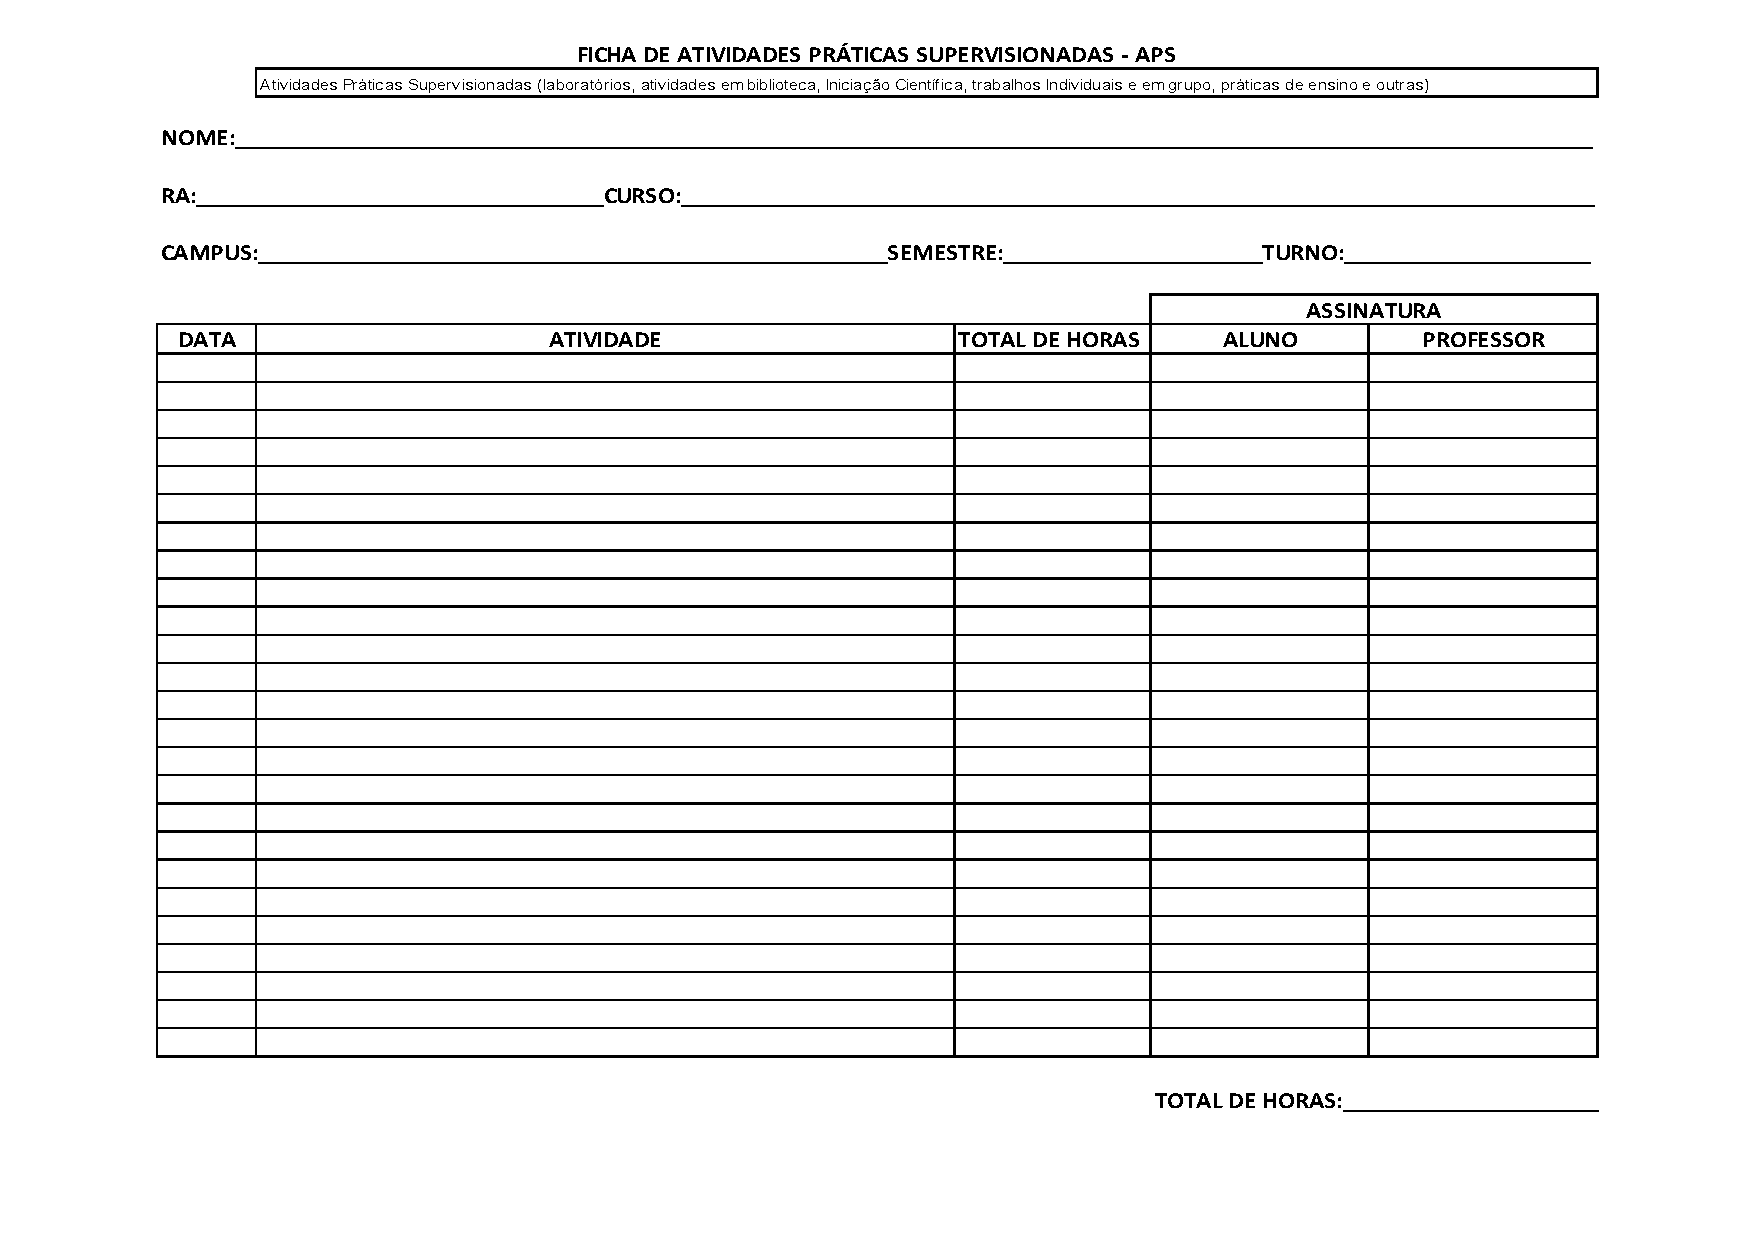
\includepdf[landscape=true]{ficha_atividades.pdf}




















\end{document}
